\chapter{VMESS, VLESS, and Trojan Protocols: Deep Dive}

This chapter provides comprehensive coverage of the three major proxy protocols implemented in Xray-core: VMESS, VLESS, and Trojan. We examine their design principles, authentication mechanisms, encryption schemes, packet structures, and implementation details with mathematical formulations and code examples.

\section{VMESS Protocol}

VMESS (Versatile Message Stream) is a custom protocol designed for high-performance proxy communication with strong security guarantees. It uses time-based authentication and supports multiple encryption methods.

\subsection{Protocol Overview}

VMESS is a stateful protocol that requires:
\begin{itemize}
    \item \textbf{UUID}: 16-byte unique identifier for authentication
    \item \textbf{Time Synchronization}: System time must be within ±120 seconds of UTC
    \item \textbf{alterId}: Legacy compatibility parameter (deprecated in newer versions)
    \item \textbf{Security Type}: Encryption method (AES-128-GCM, ChaCha20-Poly1305, None, Auto)
\end{itemize}

\subsection{VMESS Handshake Process}

The VMESS handshake consists of two phases: request header and response header.

\subsubsection{Request Header Structure}

The request header contains authentication and routing information:

\begin{verbatim}
// From Xray-core: proxy/vmess/encoding/client.go
type RequestHeader struct {
    Version  byte              // Protocol version (1)
    IV       [16]byte          // Random initialization vector
    Key      [16]byte          // Random encryption key
    V        byte              // Response authentication byte
    Option   byte              // Protocol options
    Padding  byte              // Padding length
    Security SecurityType      // Encryption method
    Command  RequestCommand    // TCP, UDP, or Mux
    Address  net.Address       // Destination address
    Port     net.Port          // Destination port
}
\end{verbatim}

\subsubsection{Request Header Generation}

\begin{verbatim}
// From Xray-core: proxy/vmess/encoding/client.go
func (c *ClientSession) EncodeRequestHeader(header *protocol.RequestHeader, writer io.Writer) error {
    buffer := buf.New()
    
    // Generate random bytes for IV, Key, and V
    randomBytes := make([]byte, 33) // 16 + 16 + 1
    rand.Read(randomBytes)
    requestBodyIV := randomBytes[:16]
    requestBodyKey := randomBytes[16:32]
    responseHeader := randomBytes[32]
    
    // Write header components
    buffer.WriteByte(Version)              // Version = 1
    buffer.Write(requestBodyIV[:])        // 16 bytes IV
    buffer.Write(requestBodyKey[:])        // 16 bytes Key
    buffer.WriteByte(responseHeader)       // Response auth byte
    buffer.WriteByte(byte(header.Option))  // Options
    
    // Security and padding
    paddingLen := dice.Roll(16)  // Random padding 0-15
    security := byte(paddingLen<<4) | byte(header.Security)
    buffer.Write([]byte{security, 0, byte(header.Command)})
    
    // Destination address and port
    if header.Command != protocol.RequestCommandMux {
        addrParser.WriteAddressPort(buffer, header.Address, header.Port)
    }
    
    // Padding
    if paddingLen > 0 {
        buffer.ReadFullFrom(rand.Reader, int32(paddingLen))
    }
    
    // FNV-1a hash for integrity
    fnv1a := fnv.New32a()
    fnv1a.Write(buffer.Bytes())
    hashBytes := buffer.Extend(4)
    fnv1a.Sum(hashBytes[:0])
    
    // Encrypt header with VMess AEAD
    fixedLengthCmdKey := account.ID.CmdKey()  // 16 bytes from UUID
    vmessout := vmessaead.SealVMessAEADHeader(fixedLengthCmdKey, buffer.Bytes())
    
    writer.Write(vmessout)
    return nil
}
\end{verbatim}

\subsection{VMESS AEAD Encryption}

VMESS uses Authenticated Encryption with Associated Data (AEAD) for header encryption. The encryption key is derived from the UUID:

\[
K_{\text{cmd}} = \text{MD5}(\text{UUID} || \text{"c48619fe-8f02-49e0-b9e9-edf163eab5d6"})
\]

The header is encrypted using AES-128-GCM:

\[
(C, \text{Tag}) = \text{AES-128-GCM.Encrypt}(K_{\text{cmd}}, \text{IV}, \text{Header}, \text{AAD})
\]

\begin{verbatim}
// From Xray-core: proxy/vmess/aead/encrypt.go
func SealVMessAEADHeader(key [16]byte, data []byte) []byte {
    // Generate random nonce
    nonce := make([]byte, 12)
    rand.Read(nonce)
    
    // Derive encryption key
    kdfNonce := KDF(key[:], KDFSaltConstVMessHeaderPayloadIVAEADKey)[:16]
    kdfIV := KDF(key[:], KDFSaltConstVMessHeaderPayloadAEADIV)[:12]
    
    // Encrypt with AES-128-GCM
    aead := crypto.NewAesGcm(kdfNonce)
    encrypted := aead.Seal(nil, kdfIV, data, nil)
    
    // Prepend nonce
    return append(nonce, encrypted...)
}
\end{verbatim}

\subsection{VMESS Body Encryption}

After the handshake, the request body is encrypted using the negotiated security type:

\subsubsection{AES-128-GCM}

\[
K_{\text{body}} = \text{SHA-256}(\text{requestBodyKey})[0:16]
\]
\[
\text{IV}_{\text{body}} = \text{SHA-256}(\text{requestBodyIV})[0:16]
\]

Each chunk is encrypted independently:
\[
(C_i, \text{Tag}_i) = \text{AES-128-GCM.Encrypt}(K_{\text{body}}, \text{IV}_{\text{body}} + i, P_i, \text{Size}_i)
\]

\subsubsection{ChaCha20-Poly1305}

\[
K_{\text{chacha}} = \text{MD5}(\text{requestBodyKey}) || \text{MD5}(\text{MD5}(\text{requestBodyKey}))
\]

The key derivation:
\[
K[0:16] = \text{MD5}(\text{requestBodyKey})
\]
\[
K[16:32] = \text{MD5}(K[0:16])
\]

\begin{verbatim}
// From Xray-core: proxy/vmess/encoding/auth.go
func GenerateChacha20Poly1305Key(b []byte) []byte {
    key := make([]byte, 32)
    t := md5.Sum(b)
    copy(key, t[:])           // First 16 bytes
    t = md5.Sum(key[:16])
    copy(key[16:], t[:])      // Second 16 bytes
    return key
}
\end{verbatim}

\subsection{VMESS Response Header}

The server responds with a response header:

\begin{verbatim}
type ResponseHeader struct {
    Option  byte    // Response options
    Command byte    // Echo command
    Port    uint16  // Echo port
    Address Address // Echo address
}
\end{verbatim}

The response header is encrypted using keys derived from the request:

\[
K_{\text{resp}} = \text{SHA-256}(\text{requestBodyKey})[0:16]
\]
\[
\text{IV}_{\text{resp}} = \text{SHA-256}(\text{requestBodyIV})[0:16]
\]

\begin{figure}[h]
    \centering
    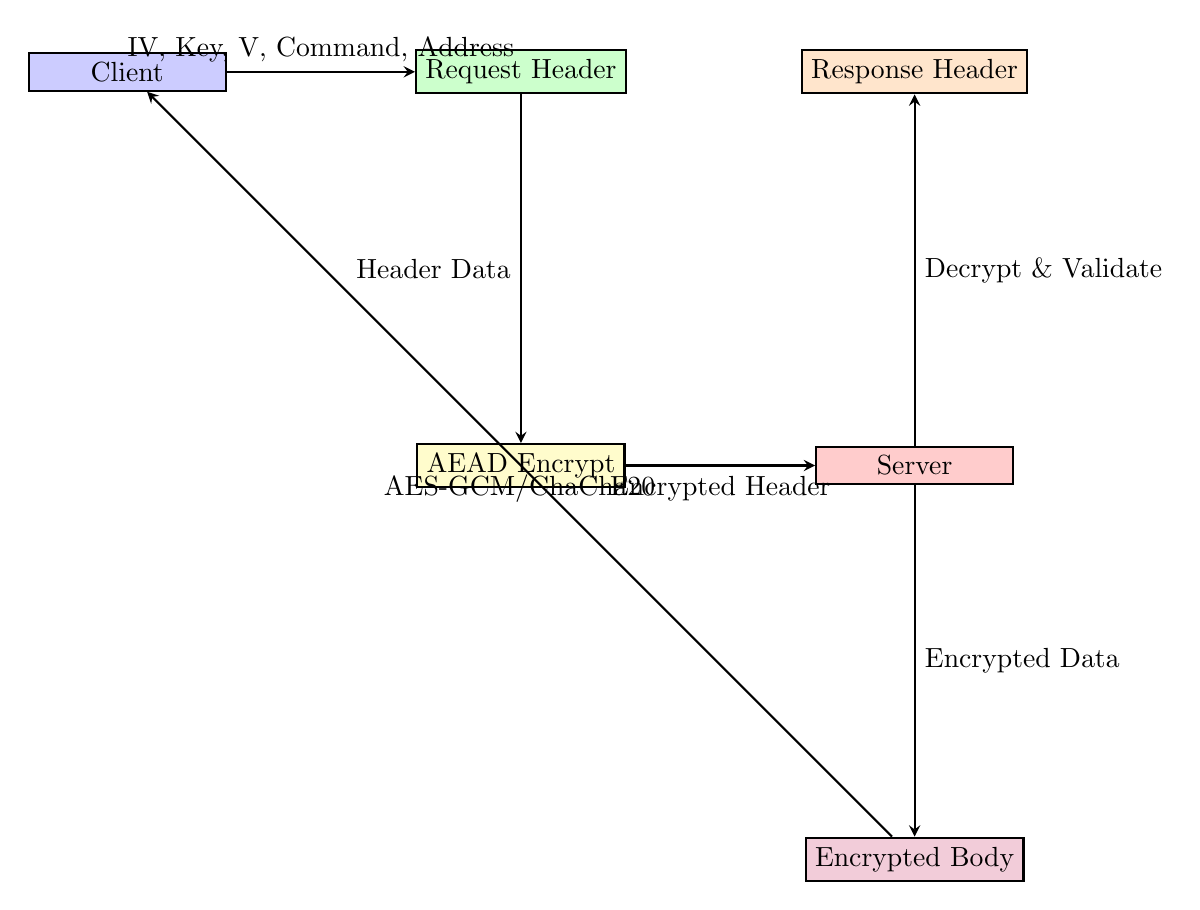
\begin{tikzpicture}[node distance=5cm,>=stealth,thick]
        \node (client) [draw, rectangle, fill=blue!20, minimum width=2.5cm] {Client};
        \node (req) [draw, rectangle, right of=client, fill=green!20, minimum width=2cm] {Request Header};
        \node (enc) [draw, rectangle, below of=req, fill=yellow!20, minimum width=2cm] {AEAD Encrypt};
        \node (server) [draw, rectangle, right of=enc, fill=red!20, minimum width=2.5cm] {Server};
        \node (resp) [draw, rectangle, above of=server, fill=orange!20, minimum width=2cm] {Response Header};
        \node (body) [draw, rectangle, below of=server, fill=purple!20, minimum width=2cm] {Encrypted Body};
        
        \draw[->] (client) -- node[above] {IV, Key, V, Command, Address} (req);
        \draw[->] (req) -- node[left] {Header Data} (enc);
        \draw[->] (enc) -- node[below] {Encrypted Header} (server);
        \draw[->] (server) -- node[right] {Decrypt \& Validate} (resp);
        \draw[->] (server) -- node[right] {Encrypted Data} (body);
        \draw[->] (body) -- node[below] {AES-GCM/ChaCha20} (client);
    \end{tikzpicture}
    \caption{VMESS Protocol Handshake and Data Flow}
\end{figure}

\subsection{VMESS Time-Based Authentication}

VMESS requires accurate system time for authentication. The server validates:

\[
|\text{ServerTime} - \text{ClientTime}| < 120 \text{ seconds}
\]

The authentication uses HMAC-SHA256:

\[
\text{Auth} = \text{HMAC-SHA256}(K_{\text{cmd}}, \text{Header} || \text{Timestamp})
\]

\subsection{VMESS Chunk Stream}

VMESS supports chunked streaming with size masking:

\[
\text{EncryptedSize} = \text{Size} \oplus \text{SHAKE-128}(\text{IV})[0:2]
\]

\begin{verbatim}
// From Xray-core: proxy/vmess/encoding/auth.go
type ShakeSizeParser struct {
    shake  sha3.ShakeHash
    buffer [2]byte
}

func (s *ShakeSizeParser) Encode(size uint16, b []byte) []byte {
    mask := s.next()  // Get 2 bytes from SHAKE-128 stream
    binary.BigEndian.PutUint16(b, mask^size)
    return b[:2]
}
\end{verbatim}

\section{VLESS Protocol}

VLESS (Versatile Lightweight Encrypted Stream) is a simplified, stateless protocol designed for better performance and flexibility. It supports advanced features like XTLS (eXtended TLS) for zero-copy optimization.

\subsection{Protocol Overview}

VLESS is simpler than VMESS:
\begin{itemize}
    \item \textbf{UUID}: 16-byte identifier (required, no alterId)
    \item \textbf{Encryption}: Optional (default: "none")
    \item \textbf{Flow}: Optional flow control (e.g., "xtls-rprx-vision")
    \item \textbf{No Time Sync}: Unlike VMESS, VLESS doesn't require time synchronization
\end{itemize}

\subsection{VLESS Request Header}

The VLESS request header is much simpler than VMESS:

\begin{verbatim}
// From Xray-core: proxy/vless/encoding/encoding.go
type RequestHeader struct {
    Version byte              // Always 0
    UUID    [16]byte          // User UUID
    Addons  *Addons           // Flow and other addons
    Command RequestCommand    // TCP, UDP, Mux, Rvs
    Address net.Address       // Destination
    Port    net.Port          // Destination port
}
\end{verbatim}

\subsubsection{Header Encoding}

\begin{verbatim}
// From Xray-core: proxy/vless/encoding/encoding.go
func EncodeRequestHeader(writer io.Writer, request *protocol.RequestHeader, requestAddons *Addons) error {
    buffer := buf.StackNew()
    
    buffer.WriteByte(request.Version)  // Version = 0
    buffer.Write(request.User.Account.(*vless.MemoryAccount).ID.Bytes())  // 16 bytes UUID
    
    // Encode addons (flow, etc.)
    EncodeHeaderAddons(&buffer, requestAddons)
    
    buffer.WriteByte(byte(request.Command))  // Command
    
    // Address and port (if not Mux/Rvs)
    if request.Command != protocol.RequestCommandMux && 
       request.Command != protocol.RequestCommandRvs {
        addrParser.WriteAddressPort(&buffer, request.Address, request.Port)
    }
    
    writer.Write(buffer.Bytes())
    return nil
}
\end{verbatim}

\subsection{VLESS Encryption (Optional)}

VLESS supports optional encryption using X25519 and ML-KEM-768:

\subsubsection{X25519 Key Exchange}

\[
\text{Client}: a \in_R [0, 2^{256}), A = aG
\]
\[
\text{Server}: B \text{ (public key)}
\]
\[
\text{Shared Secret}: S = aB = abG
\]
\[
\text{Derived Key}: K = \text{BLAKE3}(S)
\]

\subsubsection{ML-KEM-768 Post-Quantum Key Exchange}

\[
\text{Server}: (sk, pk) = \text{ML-KEM-768.KeyGen}()
\]
\[
\text{Client}: (K, ct) = \text{ML-KEM-768.Encaps}(pk)
\]
\[
\text{Server}: K' = \text{ML-KEM-768.Decaps}(sk, ct)
\]

\begin{verbatim}
// From Xray-core: proxy/vless/encryption/client.go
func (i *ClientInstance) Handshake(conn net.Conn) (*CommonConn, error) {
    // Generate IV
    iv := make([]byte, 16)
    rand.Read(iv)
    
    // Perform key exchange for each relay
    for j, k := range i.NfsPKeys {
        if k, ok := k.(*ecdh.PublicKey); ok {
            // X25519 key exchange
            privateKey, _ := ecdh.X25519().GenerateKey(rand.Reader)
            nfsKey, err := privateKey.ECDH(k)
            // ...
        } else if k, ok := k.(*mlkem.EncapsulationKey768); ok {
            // ML-KEM-768 key exchange
            nfsKey, ciphertext := k.Encapsulate()
            // ...
        }
    }
    
    // Create AEAD from derived keys
    nfsAEAD := NewAEAD(iv, nfsKey, useAES)
    // ...
}
\end{verbatim}

\subsection{VLESS XTLS Flow}

XTLS (eXtended TLS) is a zero-copy optimization that allows direct splicing of TLS connections:

\subsubsection{xtls-rprx-vision Flow}

The "xtls-rprx-vision" flow enables:
\begin{itemize}
    \item \textbf{Zero-Copy}: Direct memory copy without encryption/decryption
    \item \textbf{TLS 1.3 Only}: Requires TLS 1.3 for security
    \item \textbf{Traffic Obfuscation}: Makes traffic patterns less distinguishable
\end{itemize}

\begin{verbatim}
// From Xray-core: proxy/vless/outbound/outbound.go
if requestAddons.Flow == vless.XRV {
    // XTLS Vision flow
    ob.CanSpliceCopy = 2  // Enable zero-copy
    
    // Access TLS connection's internal buffers
    if tlsConn, ok := iConn.(*tls.Conn); ok {
        if tlsConn.ConnectionState().Version != gotls.VersionTLS13 {
            return errors.New("XTLS requires TLS 1.3")
        }
        // Direct access to TLS input buffer for zero-copy
        input = (*bytes.Reader)(unsafe.Pointer(p + i.Offset))
        rawInput = (*bytes.Buffer)(unsafe.Pointer(p + r.Offset))
    }
}
\end{verbatim}

\begin{figure}[h]
    \centering
    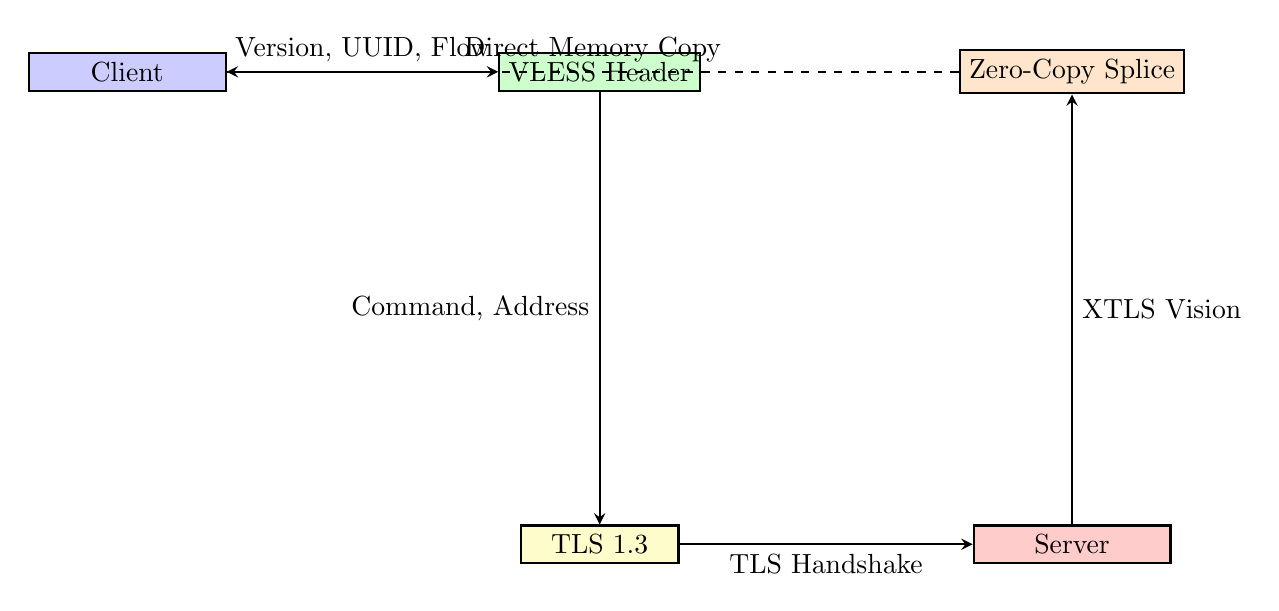
\begin{tikzpicture}[node distance=6cm,>=stealth,thick]
        \node (client) [draw, rectangle, fill=blue!20, minimum width=2.5cm] {Client};
        \node (header) [draw, rectangle, right of=client, fill=green!20, minimum width=2cm] {VLESS Header};
        \node (tls) [draw, rectangle, below of=header, fill=yellow!20, minimum width=2cm] {TLS 1.3};
        \node (server) [draw, rectangle, right of=tls, fill=red!20, minimum width=2.5cm] {Server};
        \node (splice) [draw, rectangle, above of=server, fill=orange!20, minimum width=2cm] {Zero-Copy Splice};
        
        \draw[->] (client) -- node[above] {Version, UUID, Flow} (header);
        \draw[->] (header) -- node[left] {Command, Address} (tls);
        \draw[->] (tls) -- node[below] {TLS Handshake} (server);
        \draw[->] (server) -- node[right] {XTLS Vision} (splice);
        \draw[->, dashed] (splice) -- node[above] {Direct Memory Copy} (client);
    \end{tikzpicture}
    \caption{VLESS Protocol with XTLS Vision Flow}
\end{figure}

\subsection{VLESS Response Header}

The VLESS response header is minimal:

\begin{verbatim}
type ResponseHeader struct {
    Version byte    // Echo request version
    Addons  *Addons // Response addons
}
\end{verbatim}

\section{Trojan Protocol}

Trojan is a simple, stateless protocol that mimics HTTPS traffic. It uses password-based authentication and relies on TLS for encryption.

\subsection{Protocol Overview}

Trojan is designed to be indistinguishable from HTTPS:
\begin{itemize}
    \item \textbf{Password}: SHA-224 hash of user password (56 bytes)
    \item \textbf{TLS Required}: All traffic must be wrapped in TLS
    \item \textbf{Simple Header}: Minimal protocol overhead
    \item \textbf{No Encryption}: Trojan itself doesn't encrypt; relies on TLS
\end{itemize}

\subsection{Trojan Request Header}

The Trojan request header is extremely simple:

\begin{verbatim}
// From Xray-core: proxy/trojan/protocol.go
type RequestHeader struct {
    Password [56]byte    // SHA-224 hash of password
    CRLF     [2]byte     // \r\n
    Command  byte        // 1 = TCP, 3 = UDP
    Address  net.Address // Destination address
    Port     net.Port    // Destination port
    CRLF     [2]byte     // \r\n
}
\end{verbatim}

\subsubsection{Header Encoding}

\begin{verbatim}
// From Xray-core: proxy/trojan/protocol.go
func (c *ConnWriter) writeHeader() error {
    buffer := buf.StackNew()
    
    // Write password hash (56 bytes)
    buffer.Write(c.Account.Key)  // SHA-224 hash
    
    // Write CRLF
    buffer.Write([]byte{'\r', '\n'})
    
    // Write command (1 = TCP, 3 = UDP)
    command := commandTCP
    if c.Target.Network == net.Network_UDP {
        command = commandUDP
    }
    buffer.WriteByte(command)
    
    // Write address and port
    addrParser.WriteAddressPort(&buffer, c.Target.Address, c.Target.Port)
    
    // Write CRLF
    buffer.Write([]byte{'\r', '\n'})
    
    c.Writer.Write(buffer.Bytes())
    c.headerSent = true
    return nil
}
\end{verbatim}

\subsection{Trojan Password Authentication}

Trojan uses SHA-224 hash of the password:

\[
K = \text{SHA-224}(\text{Password})
\]

The server validates the password hash:

\begin{verbatim}
// From Xray-core: proxy/trojan/validator.go
type Validator struct {
    email sync.Map
    users sync.Map  // Key: hex string of SHA-224 hash
}

func (v *Validator) Get(hash string) *protocol.MemoryUser {
    u, _ := v.users.Load(hash)
    if u != nil {
        return u.(*protocol.MemoryUser)
    }
    return nil
}
\end{verbatim}

\subsection{Trojan UDP Protocol}

For UDP packets, Trojan uses a different format:

\begin{verbatim}
// UDP Packet Format:
// [Address][Port][Length (2 bytes)][CRLF][Payload]
func (w *PacketWriter) writePacket(payload []byte, dest net.Destination) (int, error) {
    buffer := buf.StackNew()
    
    // Write address and port
    addrParser.WriteAddressPort(&buffer, dest.Address, dest.Port)
    
    // Write payload length (2 bytes, big-endian)
    lengthBuf := [2]byte{}
    binary.BigEndian.PutUint16(lengthBuf[:], uint16(len(payload)))
    buffer.Write(lengthBuf[:])
    
    // Write CRLF
    buffer.Write([]byte{'\r', '\n'})
    
    // Write payload
    buffer.Write(payload)
    
    w.Write(buffer.Bytes())
    return len(payload), nil
}
\end{verbatim}

\begin{figure}[h]
    \centering
    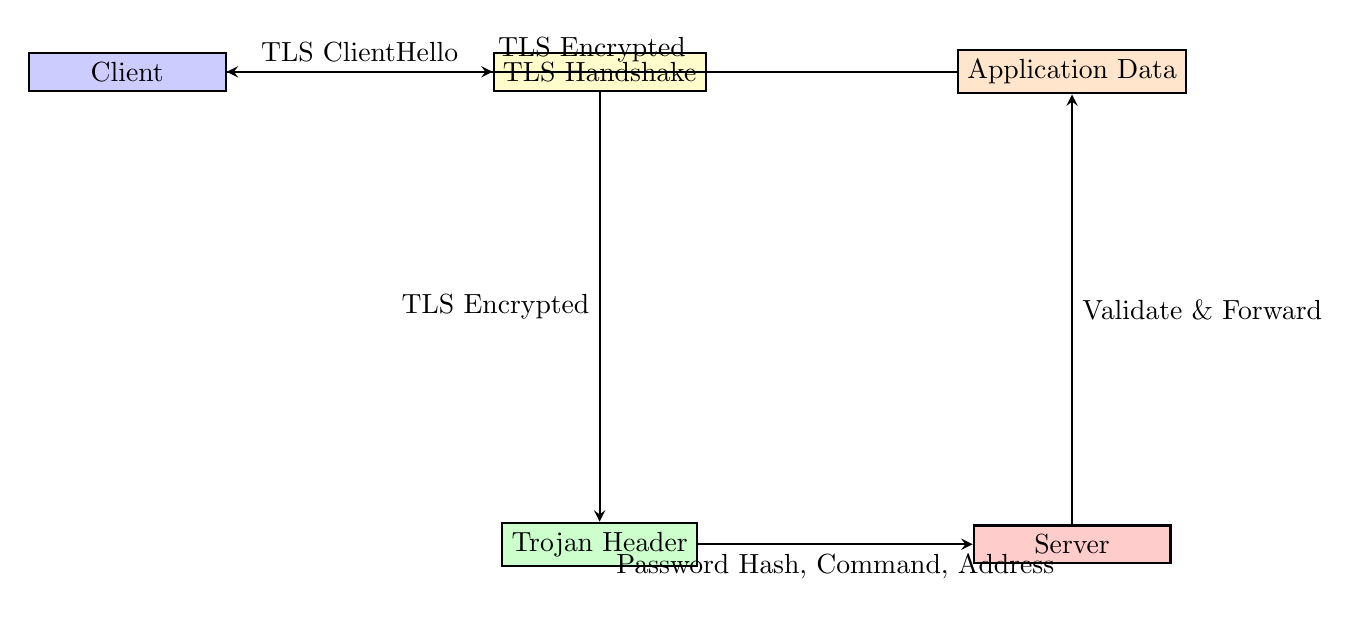
\begin{tikzpicture}[node distance=6cm,>=stealth,thick]
        \node (client) [draw, rectangle, fill=blue!20, minimum width=2.5cm] {Client};
        \node (tls) [draw, rectangle, right of=client, fill=yellow!20, minimum width=2cm] {TLS Handshake};
        \node (header) [draw, rectangle, below of=tls, fill=green!20, minimum width=2cm] {Trojan Header};
        \node (server) [draw, rectangle, right of=header, fill=red!20, minimum width=2.5cm] {Server};
        \node (data) [draw, rectangle, above of=server, fill=orange!20, minimum width=2cm] {Application Data};
        
        \draw[->] (client) -- node[above] {TLS ClientHello} (tls);
        \draw[->] (tls) -- node[left] {TLS Encrypted} (header);
        \draw[->] (header) -- node[below] {Password Hash, Command, Address} (server);
        \draw[->] (server) -- node[right] {Validate \& Forward} (data);
        \draw[->] (data) -- node[above] {TLS Encrypted} (client);
    \end{tikzpicture}
    \caption{Trojan Protocol Flow (TLS-Wrapped)}
\end{figure}

\section{Protocol Comparison}

\subsection{Feature Comparison}

\begin{table}[h]
\centering
\begin{tabular}{|l|c|c|c|}
\hline
\textbf{Feature} & \textbf{VMESS} & \textbf{VLESS} & \textbf{Trojan} \\
\hline
Authentication & UUID + Time & UUID & Password Hash \\
Time Sync Required & Yes (±120s) & No & No \\
Encryption & Multiple (AES-GCM, ChaCha20) & Optional & TLS Only \\
Header Size & ~50-100 bytes & ~20-30 bytes & ~70 bytes \\
Stateful & Yes & No & No \\
Zero-Copy (XTLS) & No & Yes (Vision) & No \\
Post-Quantum & No & Yes (ML-KEM-768) & No \\
Complexity & High & Medium & Low \\
\hline
\end{tabular}
\caption{Protocol Feature Comparison}
\end{table}

\subsection{Performance Characteristics}

\subsubsection{VMESS}
\begin{itemize}
    \item \textbf{Overhead}: ~50-100 bytes per connection (header)
    \item \textbf{Encryption}: AES-128-GCM or ChaCha20-Poly1305
    \item \textbf{Latency}: Higher due to time-based authentication
    \item \textbf{Throughput}: Good, but not optimal
\end{itemize}

\subsubsection{VLESS}
\begin{itemize}
    \item \textbf{Overhead}: ~20-30 bytes per connection (minimal header)
    \item \textbf{Encryption}: Optional, can use TLS or custom encryption
    \item \textbf{Latency}: Lower (no time sync requirement)
    \item \textbf{Throughput}: Excellent with XTLS Vision (zero-copy)
\end{itemize}

\subsubsection{Trojan}
\begin{itemize}
    \item \textbf{Overhead}: ~70 bytes per connection (header + TLS)
    \item \textbf{Encryption}: TLS (typically TLS 1.3)
    \item \textbf{Latency}: Low (simple protocol)
    \item \textbf{Throughput}: Good (TLS hardware acceleration)
\end{itemize}

\section{Security Analysis}

\subsection{VMESS Security}

\begin{itemize}
    \item \textbf{Authentication}: Strong (UUID + time-based)
    \item \textbf{Encryption}: Strong (AES-128-GCM, ChaCha20-Poly1305)
    \item \textbf{Forward Secrecy}: Limited (session keys derived from UUID)
    \item \textbf{Traffic Analysis}: Moderate resistance (padding, chunk masking)
\end{itemize}

\subsection{VLESS Security}

\begin{itemize}
    \item \textbf{Authentication}: Moderate (UUID only)
    \item \textbf{Encryption}: Strong (when enabled, supports post-quantum)
    \item \textbf{Forward Secrecy}: Excellent (X25519 + ML-KEM-768)
    \item \textbf{Traffic Analysis}: Good resistance (XTLS Vision obfuscation)
\end{itemize}

\subsection{Trojan Security}

\begin{itemize}
    \item \textbf{Authentication}: Weak (password hash only)
    \item \textbf{Encryption}: Strong (TLS, typically TLS 1.3)
    \item \textbf{Forward Secrecy}: Excellent (TLS 1.3 provides PFS)
    \item \textbf{Traffic Analysis}: Excellent (indistinguishable from HTTPS)
\end{itemize}

\section{Implementation Details}

\subsection{VMESS Session Management}

VMESS maintains session state for encryption:

\begin{verbatim}
// From Xray-core: proxy/vmess/encoding/client.go
type ClientSession struct {
    requestBodyKey  [16]byte
    requestBodyIV   [16]byte
    responseBodyKey [16]byte
    responseBodyIV  [16]byte
    responseReader  io.Reader
    responseHeader  byte
}
\end{verbatim}

\subsection{VLESS Connection Reuse}

VLESS supports connection pre-connection for reduced latency:

\begin{verbatim}
// From Xray-core: proxy/vless/outbound/outbound.go
if h.testpre > 0 {
    // Pre-connect connections in background
    h.preConns = make(chan *ConnExpire)
    for range h.testpre {
        go func() {
            conn, _ := dialer.Dial(ctx, rec.Destination)
            h.preConns <- &ConnExpire{Conn: conn, Expire: time.Now().Add(2 * time.Minute)}
        }()
    }
}
\end{verbatim}

\subsection{Trojan Validator}

Trojan uses a hash map for fast password lookup:

\begin{verbatim}
// From Xray-core: proxy/trojan/validator.go
type Validator struct {
    email sync.Map  // Email -> User mapping
    users sync.Map  // SHA-224 hash -> User mapping
}

func (v *Validator) Add(u *protocol.MemoryUser) error {
    key := hexString(u.Account.(*MemoryAccount).Key)  // SHA-224 hash as hex
    v.users.Store(key, u)
    return nil
}
\end{verbatim}

\section{Summary}

This chapter covered the three major proxy protocols:

\begin{itemize}
    \item \textbf{VMESS}: Feature-rich protocol with time-based authentication, multiple encryption methods, and chunk masking
    \item \textbf{VLESS}: Simplified protocol with optional encryption, XTLS support for zero-copy, and post-quantum key exchange
    \item \textbf{Trojan}: Simple protocol that mimics HTTPS, uses password authentication, and relies on TLS for encryption
\end{itemize}

Each protocol has its strengths:
\begin{itemize}
    \item \textbf{VMESS}: Best for compatibility and feature support
    \item \textbf{VLESS}: Best for performance and modern features
    \item \textbf{Trojan}: Best for traffic obfuscation and simplicity
\end{itemize}

Understanding these protocols is essential for:
\begin{itemize}
    \item Choosing the right protocol for your use case
    \item Debugging connection issues
    \item Optimizing performance
    \item Implementing protocol extensions
\end{itemize}

